\chapter{Storage System Design} \label{chapWhDesign}

This section is about warehouse design, i.e. the design from scratch or the redesign of an existing storage system ~\cite{Ashayeri1985, VanGils2017b} . This activity involves many decision problems belonging to different classes. In practice, these problems are approached in sequence, enlarging the focus of the decision from stock keeping units (SKUs), to storage areas to handling areas ~\cite{Accorsi2012, Baker2009, Dotoli2015, Park1989, Tufano2019,Yoon1996}. Figure \ref{fig_warehouse_design} identifies the hierarchical procedure used in this chapter, according to the definition of logistics problems introduced in \ref{secDecisionPatterns}. SKU are the parts stored within the storage system. Same SKUs has the same properties (e.g. id, weight, volume, package). Storage areas are a set of storage locations of the warehouse having a similar storage technology (e.g. served by forklifts, automated guided vehicle (AGV), automated storage and retrieval systems (AS/RS)). Handling areas are sets of storage areas, processing areas (e.g. packing, quality control, inbound and outbound areas), and edges (i.e. aisles connecting all these areas).

% INSERT fig_warehouse_design
\begin{figure}[hbt!]
\centering
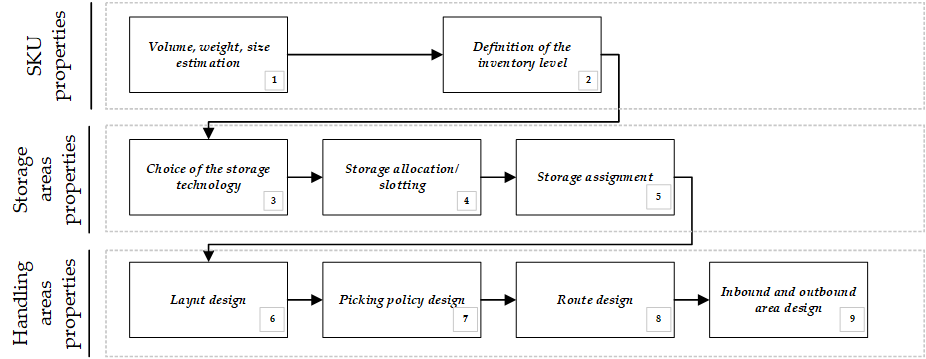
\includegraphics[width=0.9\textwidth]{SectionWarehouses/design_figures/fig_warehouse_design.png}
\captionsetup{type=figure}
\caption{Hierarchical procedure for storage system design.}
\label{fig_warehouse_design}
\end{figure}

The hierarchical procedure identifies nine decision problems:
\begin{enumerate}
    \item The estimation of weights and sizes for all the SKUs of the storage system;
    \item The definition of the inventory level for each SKU;
    \item The choice of the storage technology for each set of SKUs;
    \item The allocation of storage space to SKUs;
    \item The assignment (also known as “slotting”) of SKUs to storage locations;
    \item The design of the layout of a handling area;
    \item The definition of the picking policies (e.g. single order/batching/zoning);
    \item The definition of the routing policy (i.e. returns; traversal);
    \item The design of the inbound and outbound areas.

\end{enumerate}

The following paragraphs introduce model- and data-driven methods to address these problems.

\section{Weight and size estimation (P1)}
The knowledge of the features of the SKUs is the first step to design a storage system adequately. It may appear evident that companies must know everything about their parts. Nevertheless, the SKU master file of a warehouse management system (WMS) is easily full of null values. The most important indicator to design a storage system is the volume of its SKUs; this value is often unknown due to the labour-intensive activity to measure the dimensions of thousands of SKUs. In practice, a warehouse designer needs to know the size (i.e. length, height and width), and the weight of an SKU.

\subsection{Model-driven methods ()}
When sizes and weights are unknown for all the SKUs of a storage system, on-field measurement is the only possibility to start generating this data. A scale is used to measure the weight; the length, height, and width of an SKU are used to define its volume. When dealing with the measurement of the volume of the SKUs of an existing storage system, an approximate procedure exist. Let $v_i$ be the volume of SKU $i$ to measure. We estimate the volume $v_i$ by using  $\widehat{v_i}=\frac{1}{card(j:n_{ij}>0)}\ \sum_{j:n_{ij>0}}\left[\frac{V_j\ \eta_j}{n_{ij}}\right]$ where  $\eta_j\in[0,1]$ is the percentage saturation of each storage location $j$, and $n_{ij}$ is the number of SKUs $i$ stored in each location $j$. $V_j$ is the volume of the storage location $j$. This way, it is possible to measure a single storage location $j$, to observe the storage locations to estimate $\eta_j$, and to consider the number of SKUs $n_{ij}$ obtained, for example, from the inventory of the WMS. This procedure is approximated but faster than measuring thousands of SKUs and it provides information on how much the volumes of SKUs $i$ are different.

\subsection{Data-driven methods ()}
When a feature (e.g. the volume) is given for a subset of SKUs of the SKU master file, this procedure can be used to extend the properties of the given features to the whole set of SKUs by using clustering ~\cite{Tufano2019}.\par

The description of an SKU is always recorded together with the id in the WMS. This is mainly due to avoiding errors since pickers read on their terminal the description of the SKU they have to pick. We use text mining techniques to cluster SKUs based on their description. In particular, we build a bag of words (BOW) model using the descriptions of the SKUs.\par

A BOW is a frequency analysis on text strings. The BOW model counts the number of occurrences of each word, giving higher importance to the strings occurring the most. It is necessary to clean the input strings separating words (e.g. removing \_ and - characters) and removing special characters (i.e., +, /, |, ”,  ’, . characters), in order to make the BOW model work properly. BOW defines a vocabulary of the storage system (SSV) which contains the one single words or a couple of words occurring the most. It is recommendable to set a threshold on the minimum number of occurrences for a word to enter the SSV (e.g., at least ten occurrences among all the descriptions) to prevent having huge and meaningless SSVs. Finally, each SKU is associated with a set $B_i$ i.e., containing each word of the SSV contained by the description of the SKU $i$.\par

At this stage, unsupervised learning methods are used to find patterns among SKUs descriptions based on the values of the sets $B_i$. A matrix $M$ is defined to measure the similarity between each couple of SKUs (e.g. SKUs $i$, and $h$) based on the value of a similarity index (e.g. the Jaccard index) calculated on $B_i$,$B_h$. A hierarchical clustering algorithm (e.g. complete linkage CLINK, single linkage SLINK or average linkage UPGMA) is applied on $M$ to define clusters of SKUs. Once clusters are defined, the given properties of an SKU are extended to all the SKUs of a cluster. If the features are known for many SKUs within the same cluster, their value is averaged before extending to the other SKUs.

\section{Definition of the inventory level (P5)} \label{secInventoryDesign}
The definition of the level of inventory of a storage system is a crucial decision to reduce the storage costs of the storage system ~\cite{Cormier1999,Cormier1992,Goh2001, Hung1984, Levy1974, Lowe1979, Rao1998, Rosenblatt1984, Rosenblatt1988, White1971}. The definition of the inventory level is based on the statistical analysis of previous observation of the inventory values. For this reason, we only introduce data-driven methods.
%\clearpage
\bibliographystyle{ieeetr}
\bibliography{SectionWarehouses/design_ref}
